\chapter{Manual del programador}
\label{Anexo:ManualProgramador}
Este capítulo tiene como objetivo facilitar el acercamiento al proyecto por parte de un programador externo. Siguiendo los apartados desarrollados a continuación, tendrá la información necesaria para realizar modificaciones o ampliar el trabajo ya realizado.

\section{Requisitos hardware recomendados}
Debido a que se realizan ejecuciones muy costosas en local, los requisitos recomendados para este proyecto son bastante exigentes.
En primer lugar, dado que las imágenes \textit{Galaxy} son muy pesadas (del orden de los 10 GB) y los datos generados por el workflow también son considerables, se recomienda un espacio libre en disco de unos 20 GB para una utilización cómoda de la aplicación.
En cuanto a la memoria RAM, se recomienda utilizar una capacidad mayor que el tamaño de los datos de entrada. Esto se debe a la forma de ejecución de algunas herramientas del workflow, que necesitan cargar todas las secuencias a la vez en memoria. En nuestro caso se han utilizado 16 GB de RAM para un conjunto de datos de entrada de 10 GB.
El caso del procesador no es tan limitante como el anterior, sin embargo, definirá el tiempo total de ejecución. El caso de prueba mencionado anteriormente se ha ejecutado con un procesador Intel i7-9700K, con un tiempo de ejecución de unas 3 horas. Por lo tanto, cualquier procesador de un sistema de 64 bits será capaz de realizar la ejecución.

\section{Requisitos software necesarios}
El proyecto está enfocado a ser ejecutado en un sistema \textit{Ubuntu}, en concreto, se ha utilizado la versión 18.04.1. Sin embargo, desde la perspectiva de un desarrollador, con unos cambios menores puede llegar a adaptarse a cualquier sistema sin demasiado esfuerzo.
    \subsection{\textit{Docker}}
    Docker es un sistema de código abierto basado en contenedores que permiten el despliegue de aplicaciones dentro de sí mismos. Los contenedores ofrecen la posibilidad de empaquetar todo el software necesario para ejecutar nuestra aplicación, ofreciendo un modo de virtualización mucho más aislado y ligero que el uso de máquinas virtuales. Además, se mantiene la seguridad de que nuestra aplicación será utilizable en cualquier sistema en el que se pueda realizar esta virtualización.
    
    Durante el desarrollo del proyecto se ha utilizado la versión 18.09.1 de \textit{Docker}, por lo que se recomienda la instalación de una versión igual o superior a esta. El proceso para instalar \textit{Docker} en \textit{Ubuntu} no es complejo y en la propia web encontramos una guía de instalación \footnote{https://docs.docker.com/install/linux/docker-ce/ubuntu/}.


    \subsection{Python}
    \textit{Python} es uno de los lenguajes de programación más utilizados en el mundo. Es un lenguaje interpretado, de alto nivel, de propósito general, de código abierto y multiplataforma. Su facilidad de uso y comprensión han hecho que su crecimiento haya sido notable en los últimos años, especialmente en investigación.
    Algunas de las funcionalidades del desarrollo se han creado a través de \textit{Python 3.7.2}. Se recomienda la utilización de una versión superior a 3.6. Además de \textit{Python} estándar, se han utilizado varias librerías:
        \begin{description}
            
            \item[\textit{Bioblend} 0.12.0] es un paquete que posibilita la interacción con la API de \textit{Galaxy}, permitiendo actuar sobre la instancia desplegada en \textit{Docker}.
            
            \item[\textit{Pandas} 0.24] permite la utilización de nuevas estructuras y métodos para el análisis de datos. Se utiliza en este caso para tareas simples, como gestionar ficheros de tipo \textit{tabular}, \textit{csv} y \textit{xls}.
            
            \item[\textit{Numpy} 1.15.4] es uno de los paquetes más utilizados de Python, facilitando gran variedad de funciones matemáticas. En el caso de \textit{Numpy} es importante utilizar esta versión en concreto, ya que en este momento la versión actual (1.16.0) pressenta incompatibilidades con otra de las librerías instaladas, \textit{PyInstaller}.
            
            \item[\textit{PyInstaller} 3.4] es una utilidad que permite generar ejecutables a partir del código \textit{Python} para así evitar las instalaciones, tanto del propio \textit{Python}, como de sus dependencias.
        
        \end{description}
    
        Las instalaciones de todas estas librerías pueden realizarse sin problema desde \textit{pip} con el comando \textit{<<pip install librería\_deseada>>}.

\section{Estructura del proyecto}
\begin{figure}
    \begin{center}
      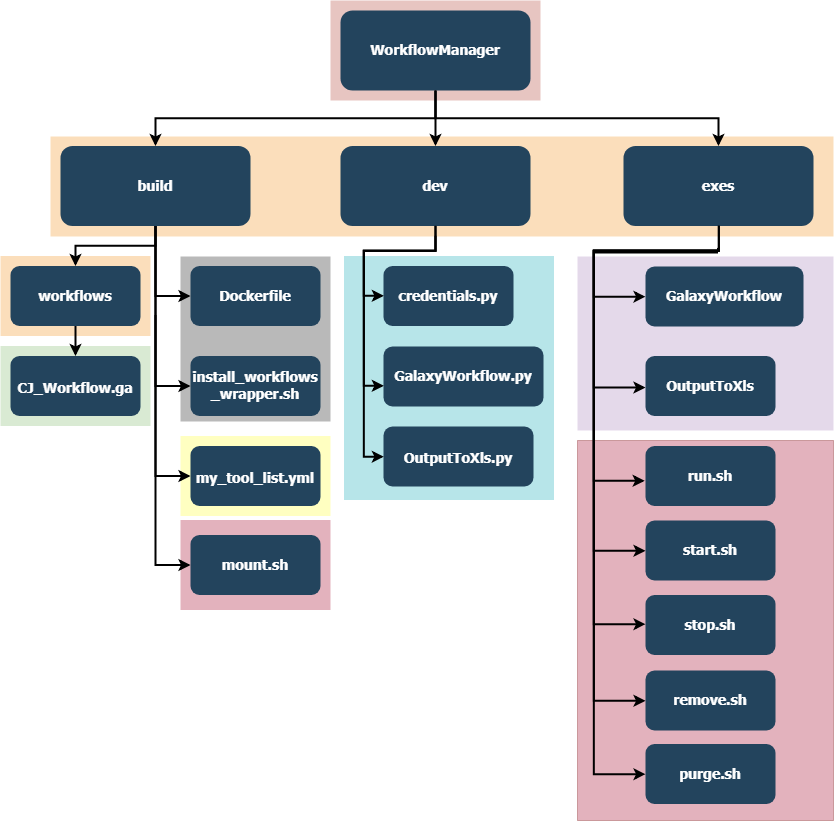
\includegraphics[scale=0.4]{images/FolderStructure.png}
      \caption{Contenido del proyecto}
      \label{fig:ContenidoDelProyecto}
    \end{center}
\end{figure}

\subsection{Directorio de ensamblado: \textit{<<build>>}}
Todos los componentes necesarios para construir la imagen \textit{Docker} de \textit{Galaxy} se encuentran en el directorio <<build>>. El fichero más relevante es <<Dockerfile>>, que contiene todas las directivas que indican cómo construir esta imagen. En concreto, realiza algunas variaciones sobre una imagen ya existente. Para realizar este montaje, será necesario el fichero <<mount.sh>>, que se encargará de utilizar las instrucciones de <<Dockerfile>> para construir y desplegar la imagen en un contenedor \textit{Docker}. Los dos ficheros <<install\_workflows\_wrapper.sh>> y <<my\_tool\_list.yml>> son utilidades para la instalación de workflows y herramientas de \textit{Galaxy} respectivamente. Las herramientas indicadas se instalarán desde el <<tool shed>> de \textit{Galaxy}, mientras que los workflows se encontrarán en el directorio <<workflows>>.

\subsection{Directorio de desarrollo: \textit{<<dev>>}}
Las utilidades desarrolladas en Python se almacenan en este directorio. Aquí encontramos dos ficheros principales, <<GalaxyWorkflow.py>> y <<OutputToXls.py>. El primero de ellos es el encargado de simplificar la utilización del workflow a los usuarios. Basándose en la API de \textit{Galaxy} a través del uso de la librería \textit{BioBlend}, se identifica en \textit{Galaxy} utilizando las credenciales indicadas en el fichero <<credentials.py>>. A continuación, genera nuevos historiales para almacenar los datos de entrada y los futuros datos de salida. Buscará dentro de los directorios <<Forward>> y <<Reverse>> los ficheros de las secuencias a analizar. Con ellos creará dos colecciones que servirán como entrada definitiva del workflow. Una vez ejecutado, el script se encargará de descargar los ficheros de salida de las tres últimas herramientas, que son los que en este caso se desean utilizar posteriormente.

Por su parte, el script <<OutputToXls.py>> se encargará, a través del uso de \textit{Pandas}, de crear un solo fichero <<.xls>> a partir de las salidas generadas por las herramientas \textit{Roary} y \textit{ABRicate} para facilitar el tratamiento de los datos por parte del equipo que los va a utilizar, dado que están familiarizados con \textit{Excel}.

\subsection{Directorio de ejecución: \textit{<<exes>>}}
En este directorio encontraremos, en primer lugar, los ejecutables correspondientes a los ficheros \textit{Python} del directorio <<dev>>, con el objetivo de evitar la instalación de \textit{Python} y sus dependencias al usuario. Además, se han desarrollado varios ficheros para simplificar el manejo de la imagen \textit{Galaxy} de \textit{Docker}, que simplemente contienen comandos para su instalación, arranque, parada y borrado. Se incluye un script <<purge.sh>> debido a que son frecuentes las acumulaciones de ficheros basura que acaban por ocupar demasiado espacio de almacenamiento. Este script es ejecutado desde los demás para evitar estos problemas.

\newpage \thispagestyle{empty} % Página vacía 